\chapter{Physics: Quantum Field Theories}

The Standard Model (SM) of particle physics classifies all known
{\it elementary particles}, i.e. particles with no known substructure,
and describes three fundamental forces: the electromagnetic,
weak, and strong forces. Elementary particles can be divided into
{\it matter particles} (quarks and leptons); {\it gauge bosons}, which mediate
the three aforementioned forces; and a {\it scalar boson}, the Higgs boson,
whose field interacts directly with elementary particles that thereby
acquire their mass. For each particle there exists a corresponding
antiparticle; sometimes a particle is its own antiparticle.
Figure~\ref{fig:SM} gives a schematic overview of the SM.
The SM has a long history of experimental confirmations culminating
in the 2012 discovery of the Higgs boson by the ATLAS and CMS
experiments~\cite{aad_observation_2012,chatrchyan_observation_2012}.

\begin{figure}
  \centering
  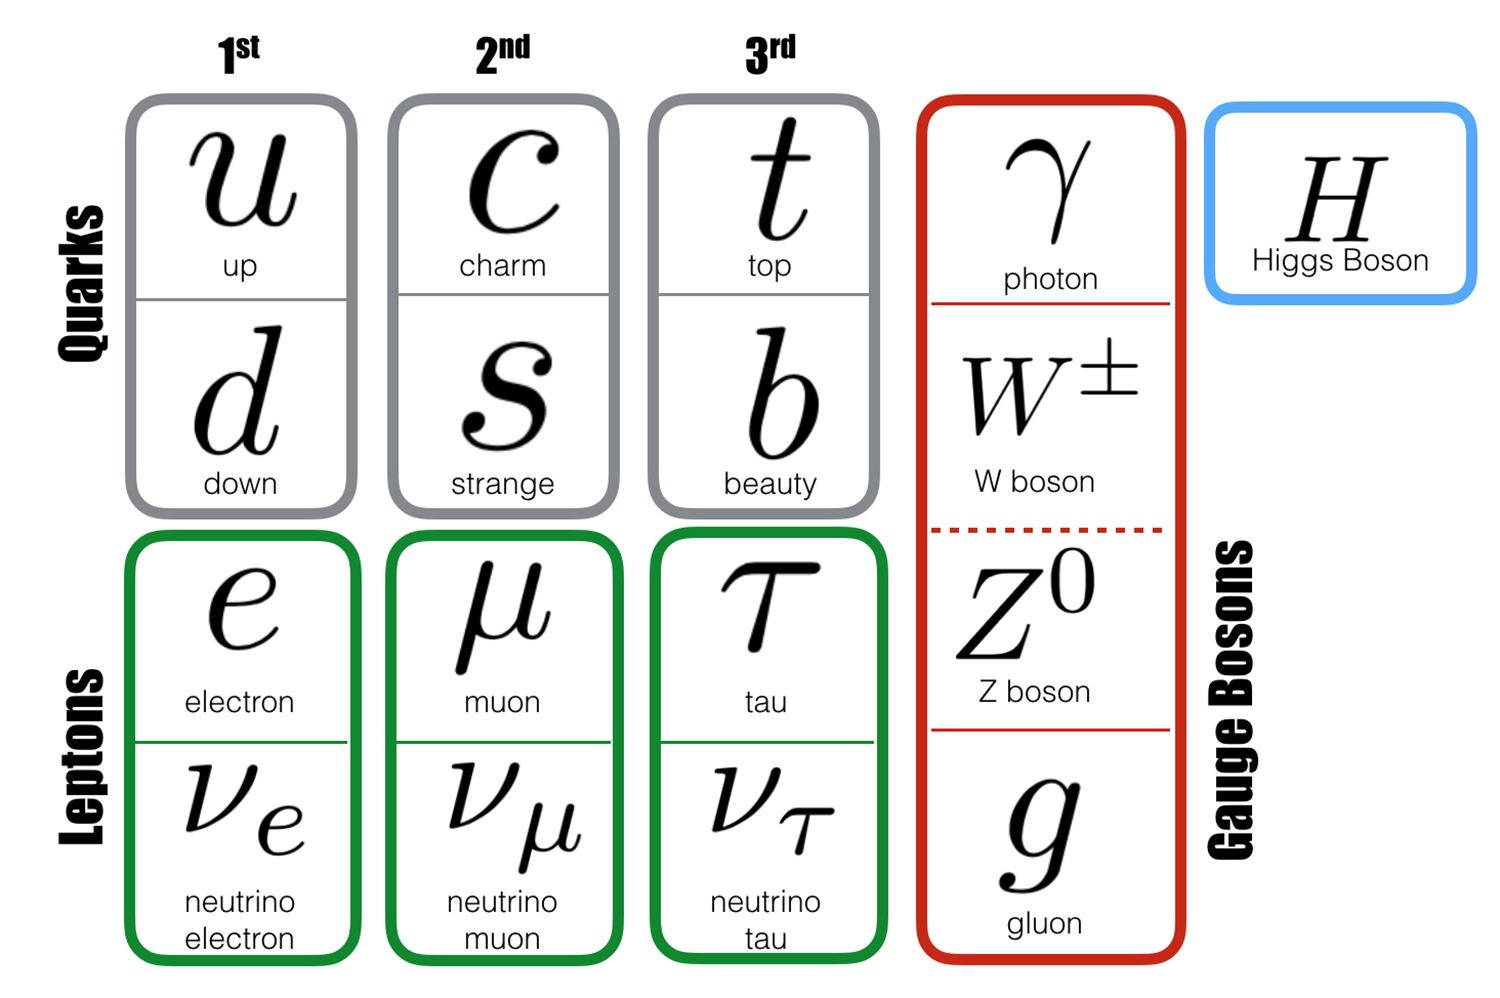
\includegraphics[width=0.95\linewidth]{figs/SM.png}
  \caption{Summary of elementary SM particles. The first three columns give
           the three generations of matter particles. Image taken
           from the Physics Institute at University of 
           Zurich~\cite{zurich_SM}.}
  \label{fig:SM}
\end{figure}

The theoretical framework underlying the SM is an example of a Quantum 
Field Theory (QFT). QFTs are consistent with both quantum mechanics and
relativity. Lattice gauge theories are a kind of QFT; therefore it is
important for the reader to know a little bit about them.

\section{The principle of stationary action}

This section follows a fairly well known and delightful lecture by Feynman
\cite{caltech}.

\section{The path integral}

\bibliographystyle{unsrtnat}
\bibliography{bibliography}
